\documentclass[12pt]{article}
% This file is in the UTF-8 encoding (codepage)
% If you see strange symbols instead of cyrillic letters,
% just switch your editor to UTF-8
% This will not affect the main part of your autoref,
% because the file is inserted as a single separate PDF
% (see below)

\usepackage [utf8]{inputenc}
\usepackage[T2A,T1]{fontenc}

\usepackage[russian]{babel}
\usepackage{amssymb,latexsym,amsmath}
\usepackage{amsfonts}
\pagestyle{plain} \textwidth=185mm \textheight=240mm
\voffset=-17mm \hoffset=-22mm
\renewcommand{\baselinestretch}{1.3}


% Для вставки подписи учёного секретаря
\usepackage{graphics}
\usepackage[dvips]{graphicx}


% Чтобы если играться с размерами, то в одном месте
\newcommand{\ScientificAssistant}[2]{
	\begin{minipage}[t]{5.9cm}
		#1\unskip:
	\end{minipage}
	\hfill
	\begin{minipage}[t]{12.5cm}
		%\raggedright
		% Отключаем переносы
		\hyphenpenalty=10000
		\exhyphenpenalty=10000
		#2
	\end{minipage}
}


\begin{document}
\large

\thispagestyle{empty}

% Это не трогаем, пишется всегда
\begin{flushright}
\textit{На правах рукописи}
\end{flushright}

\vspace{25mm}

\begin{center}
\textbf{
	Авдеев Николай Николаевич
}
\end{center}

\vspace{25mm}

\begin{center}
\textbf{\MakeUppercase{
	% Название диссертации :)
	Инвариантные банаховы пределы
}}
\end{center}

\vspace{10mm}

\begin{center}
	1.1.1. Вещественный, комплексный и функциональный анализ
	%1.1.2. Дифференциальные уравнения и математическая физика
\end{center}

\vspace{5mm}

\begin{center}
Автореферат

диссертации на соискание ученой степени кандидата

физико-математических наук
\end{center}

% И с размаху прижимаем вниз!
\vfill

\begin{center}
Москва --- 2025
%Всегда указывается город защиты - Москва
%Независимо от города написания диссертации
\end{center}


\newpage
\thispagestyle{empty}

% Поджимаем междустрочный интервал - а то не влезет!
\renewcommand{\baselinestretch}{1}
% Отключаем абзацные отступы
\setlength{\parindent}{0pt}
% Уменьшем размер шрифта :(
\fontsize{13.4}{15}\selectfont

\begin{center}
	Работа выполнена в
	% Ниже вписываем название университета
	Воронежском государственном университете
\end{center}

\vfill


\ScientificAssistant{
	Научный руководитель
}{
	Семенов Евгений Михайлович, д.ф.-м.н., профессор,
	\\
	заведующий кафедрой теории функций и геометрии
	Воронежского государственного университета
}

\vfill

\ScientificAssistant{
	Официальные оппоненты
}{
	Бородин Петр Анатольевич, д.ф.-м.н., профессор РАН,
	\\
	профессор кафедры теории функций и функционального анализа механико-математического факультета,
	\\
	ФГБОУ ВО «Московский государственный университет им. М. В. Ломоносова»
	\\
	\smallskip
	\\
	Ушакова Елена Павловна, д.ф.-м.н.,
	\\
	ведущий научный сотрудник лаборатории №45,
	\\
	ФГБУН «Институт проблем управления \\ им.~В.А.~Трапезникова Российской Академии Наук»
}

\vfill

\ScientificAssistant{
	Ведущая организация
}{
	Федеральное государственное бюджетное \\ образовательное учреждение высшего образования
	\\
	«Санкт-Петербургский государственный университет»
}



\vfill

Защита состоится TODO.2025 г. в TODO
на заседании диссертационного совета
ПДС 0200.005 при Российском университете дружбы народов имени Патриса Лумумбы
(адрес: г. Москва, ул. Орджоникидзе, д. 3).

\vspace{5mm}

С диссертацией можно ознакомиться в
Учебно-научном информационном библиотечном центре
(Научной библиотеке Российского университета дружбы народов)
по адресу: 117198, г. Москва, ул. Миклухо-Маклая, д. 6
и на сайте РУДН в сети <<Интернет>>
(https://www.rudn.ru/science/dissovet).

\vspace{10mm}

Автореферат разослан \_ \_ \_ TODO 2025 г.

\vspace{10mm}


% Прижимаем вниз с размаху!
\vfill

\noindent
\begin{minipage}{0.97\linewidth}
\noindent
Ученый секретарь диссертационного совета
\\
доктор физико-математических наук
\hfill
А. Ю. Савин
\end{minipage}
% Вставляем подпись - и впрямь "посверху"
\nolinebreak
\hspace{-6.8cm}
\begin{minipage}{0.97\linewidth}
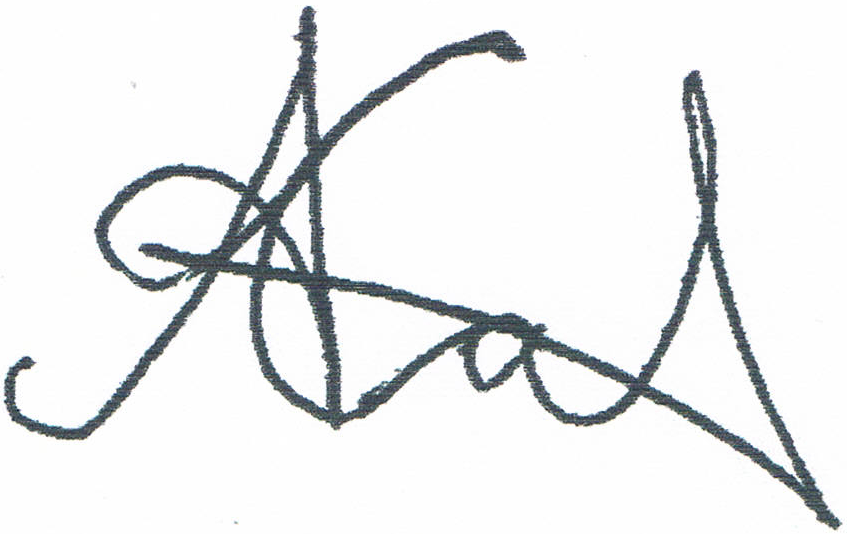
\includegraphics[width=0.10\linewidth]{Savin_signature.png}
\end{minipage}

%...но не совсем вниз...
\vspace{2cm} % по вкусу



\end{document}
